\chapter{Designing Video Games} 
\label{chap:vg}
Exergames are one type of video games. Developing a concept for an exergame require us to understand what elements a video game is build up from. There are different phases of video game development. Making a design document is mainly the one video game designers are concerned about. This design document consists of several aspects of the video game, which are important for the developer to describe. These aspects will be important in our further work.

First, we will briefly present the development phases, with emphasise on the design document. Then we will describe important elements that a video game should consist of, and that should be included in the design document.  

\section{The Design Phase}
\label{sec:designphase}
Four phases of video game development are discussed in \cite{understandingvg}: \emph{a conceptual phase}, \emph{a design phase}, \emph{a pre production phase} and \emph{a testing phase}. The first is a short description of the video game concept to sell the idea. This formulation often describes which platform the game will be build on and sometimes also concept arts. The next part of this phase is for the developers to make a \emph{game proposal} which includes market analysis, technical issues, budget projections, audiovisual style and how the game would feel to play \cite{understandingvg}. The following phase is the \emph{design phase}, which includes making a design document. The design document is what the game designers are most concerned about \cite{gamedesign}, and its goal is \emph{"[...] to fully describe and detail the gameplay of the game"} \cite{gamedesign}.  In \cite{gamedesign} they state that the design document should not include  technical details of the game design. However, in \cite{understandingvg} they include both the functional and technical specifications in the design document. The design document should at least include the story of the game, the different levels in the game world, what the players are allowed to do in the game and how they do it. In addition the design document will describe what characters and objects will be included in the game world \cite{gamedesign}. In \cite{understandingvg} they also include text, illustrations, mock-ups and concept drawings.  In \cite{gamedesign} they have separate documents for illustrations, mock-ups and concept drawings, which they describe as art bible, flow charts, and storyboards. Flow charts can be useful for visually showing decision making in the game, and is quite useful for scenarios where a lot of branching are involved. The art bible is described as \emph{"[...] the place where the look and feel of the game is comprehensively established in detail"} \cite{gamedesign}. Here it will be described what kind of art style will be used, in addition to sketches of the style. Making storyboards is a way to sketch or mock-up shots before they are filmed, and can for example be used as concept sketches to show how the game world will be seen from the player's view. 

The design document, should include the overall story-line. With a complex story line, the details can be described in what \cite{gamedesign} call the story bible.  The technical design document is in \cite{gamedesign} separated from the design document, while they join them in \cite{understandingvg}. This document focus on how the functionality will be implemented. This is out of the scope of this thesis, and will not be discussed any further. 

After the design document is finished the decision on the game engine must be made. The game engine is the software which provides the basic architecture of the game but not the concrete content, and includes handling the artificial intelligence, the audiovisuals and the physics. In addition, third-party software tools can be used to make for example some of the graphics. After the development of the design document, and the choices of the game engine and third-party software, it is common to start making working prototypes. These do not need to be playable \cite{understandingvg}. The next phases include production and testing. 

The reader should remember that the names of the different documents described in this section, in addition to the way they are divided or joined, is not the standard way of making game development documentation. This varies from developer to developer.

We will now move on to the next section, where we will describe the different elements that needs to be included in video games.

\section{Characteristics of Video Games}

Game designer Sid Meier came up with one of the most famous definitions of a game: "A game is a series of interesting choices" \cite{understandingvg}. This of course, does not apply for every video game. In \cite{understandingvg} the authors present the MDA-model, which was developed by Robin Hunicke, Marc LeBlanc and Robert Zubeck, after several workshops conducted at the "Game Developers Conference" in California between 2001 and 2004. This model divides games into three elements: \emph{mechanics}, \emph{dynamics}, and \emph{aesthetics}, and is a very useful tool for designers to understand games. \emph{Mechanics} are not something we can see or hear, but rather the rules and basic code of the game. This is for example the algorithms that lies in the ground for creating the reaction pattern of a computer-controlled character. \emph{Dynamics} are based on the mechanics and describe what events do and can occur during the gameplay, seen from the players point of view. \emph{Aesthetics} are about everything that can be experienced by the player. 

The MDA model has its limitations. It is very simple and it does not really represents how gameplay works. Also the aspects around playing experience fall outside this model, as well as the expressive side of the game. However, the writers of \cite{understandingvg} suggest that Sid Meier's definition and the MDA-model provide the most salient definitions of game, and works good for helping developers in their design work. In this thesis the \emph{aesthetics} is the most important entity, because this are all the aspects that the players experience, and it describes the entities that actually form a game. Gameplay is in \cite{understandingvg} an entity that falls under aesthetics. However, since this is a quite important entity, we will provide an own section for this. We will also describe the importance of a story, with settings and characters. First we present what aesthetics are and include. Some definitions and words used in this chapter might differ from how these words are used in "the real world". We will remind the reader that this chapter describes video games, which have virtual worlds, and that therefore some terms would not be used in the same way in real life.    


\subsection{Aesthetics}
The aesthetics describe everything that can be experienced by the player. These are the elements that actually makes the game. The aesthetics can be divided in three, namely \emph{rules}, \emph{geography and representation}, and \emph{number of players}. The rules say something about what the players can and cannot do, as well as what actions will make the score increase or decrease. The geography and representation element says something about how the video game is represented through graphics and sound. Here there are a lot of different design possibilities. The number of players is important, because there are huge differences between a single-player game and a multi-player game \cite{understandingvg}.

We will now look a little closer into the three different categories.

\subsubsection{Rules}
In \cite{understandingvg}, they distinguish between two types of rules; \emph{interplay rules} and \emph{evaluation rules}. The former are the physical laws in the gamespace, and determines what properties the different elements in the game should have, what can be done, as well as what will happen corresponding to the player input. An example of this is "What will happen when the player presses button A? Jump". The latter defines what rewarding and punishments will be given at certain actions \cite{understandingvg}. 

\subsubsection{Geography and Representation}
\label{sec:georep}
Geography and representation are about how the game is represented through graphics and sounds \cite{understandingvg}. Graphics and sounds are used to set the games environment and enhance the players enjoyment of the game, but has no effect on how the game is played.  

\emph{Graphics}\\
Graphics are needed in a videogame to in a best possible way imitate reality and enhance the player experience. This means that instead of telling out what is happening, it will be shown visually \cite{umlapproach}.
There are many aspects to consider when it comes to how the game should be represented. Table \ref{tab:graphic} shows an overview of basic geographical and representational characteristics. We will only discuss the choice of perspective, dimension and exploration in this thesis. 

\begin{table}
\centering
    \begin{tabular}{|l|l|l|l|l|}
        \hline
       \textbf{Perspective} & First person & Third person & &  \\ \hline
       \textbf{Dimension} & 2 & 3 & & \\ \hline
       \textbf{Space type} & Torus & Abstract & Free & \\ \hline
	   \textbf{Off-screen} & Dynamic & Static & None & \\ \hline
	   \textbf{Scroll} & Vertical & Horizontal & Free & None \\ \hline
	   \textbf{Exploration} & Forced & Free & None & \\
        \hline
    \end{tabular}
    \caption[Graphical Characteristics]{Basic graphical game characteristics \cite{understandingvg}.}
    \label{tab:graphic}
\end{table} 

It has to be decided if the game will be two-dimensional or three-dimensional and in first-person or third-person. Two-dimensional graphics are represented by only two coordinates and do not have any depth. This makes a very unrealistic scene. Three-dimensional graphics, on the other hand, has depth, and is therefore more realistic. All games will either have a first-person perspective, a third-person perspective, or a mix of both. In a first-person perspective, the game is played through the characters eyes, while in a third-person perspective the player can see the character she controls through the game. Games will also either have an isometric perspective or a top-down perspective. Isometric perspective is when three-dimensional objects are presented in a two-dimensional form, like in an architectural drawing, while a top-down perspective is, as the name suggest, when the scene is shown from above. The choice of perspective is important because it decides how the player will perceive the game world. It is important to choose the right perspective with the right dimension. A third-person game can be played in a two-dimensional and a three-dimensional space, while a first-person game should only be played in a three-dimensional space. Exploration says something about whether the player can move in the game at forced or desired pace. Another aspect experienced by the player is time. It is proposed to distinguish between play time and event time, where the former is the time a player uses playing the game, and the latter is the time in the game world. If play time and event time are the same, we can say that the game is played in real time. In many games it is possible to save the game, and return to the same state at a later time \cite{understandingvg}.

There are many different ways to present a game graphically. In \cite{understandingvg} they describe three different styles common for video games that were identified by Aki Järvinen: 

\begin{itemize}
\item \emph{Photorealism:} is defined as \emph{"a style of painting that tried to completely mimic photographs"} \cite{understandingvg}. There are two subcategories of photorealism: \emph{Televisualism} tries to give the same visual look as shown on the television. This is commonly used for sports games. \emph{Illusionism} is the other category. Here it is non-realistic content presented as photorealistic content. An example of this is when zombies or similar objects are presented in a way that seems like it is in real life.  
\item \emph{Caricaturism:} Here so called caricatures are used. Caricatures are drawings that presents an object by exaggerating the prominent features of the object, and often gives the feeling of a cartoon. 
\item \emph{Abstractionism:} In this category there are no real people or real-life objects involved. Instead  the game has a rather abstract form. An example of this is the well-known game Tetris. A problem with these kind of games is that they often face a hard time on the market. This is because humans mostly get attracted by the story, and it can therefore be hard to create attention just around the mechanics of the game. Therefore, it is within this category very important with the story \cite{understandingvg}. 
\end{itemize}

\emph{Sounds}\\
Sounds are important in video games for the same reasons as why graphics are important. Background music can set the atmosphere of the game, as well as give an indication on when actions will change and if the atmosphere is changing (for example from happy to sad). Sound can also be used as feedback to the player \cite{umlapproach}. There are different types of sound included in a  video game. \cite{understandingvg} distinguishes between four categories:
\emph{vocalization}, which is the voice of the characters in the game,
\emph{sound effects}, which are sounds made by the different objects in the game, \emph{ambient effects}, which are non-specific sounds that makes the atmosphere in the game, and \emph{music}, which is the game's soundtrack, and also a part of setting the atmosphere. The latter is a very important part of the game. Elements that can affect sound effects are \emph{the environment}, \emph{spatiality} and \emph{physics}. An example of how the environment can affect the sounds is what kind of floor the characters are walking on or what kind of weather conditions there are in the scene. The sound will also be affected by where in space it will come from. For example, a sound from far away sounds different from a sound close up. In addition, sound will be affected by movements. Imagine the sound of the sirens on a fast passing ambulance.

\subsubsection{Number of players}
\label{subsec:numbers}
The number of players is an important choice because it affects a number of game elements. In a single-player game artificial intelligence (AI) is important, because the player has to play against the computer and not real humans. The computer can never be as intelligent as the human brain, and generally has a very limited set of strategies. Therefore, it can be easy for an experienced player to win over the opponent. When designing multi-player games, artificial intelligence is not necessarily needed, as the player will play against other human players. In multi-player games it has to be possible to distinguish between characters. This can be done by giving them different unique features, but at the same avoid making any character superior. It is also important to facilitate social interaction between the players, like for example cooperation or competition \cite{understandingvg}. Often in multi-player games, it is possible to chat with the opponents or team members. 

\subsection{Gameplay}

"[...] gameplay is the most important element when designing a game" \cite{umlapproach}.  In \cite{understandingvg} gameplay is defined as "the game dynamics emerging from the interplay between rules and game geography". Gameplay is a result of the game's rules, while the feeling of the gameplay is influenced by the sounds and graphics. The dynamics can be of different types. They can be entertaining or they can be predictable, or they can be none of those. In a video game, everything really depends on the gameplay because it defines how the game is played. In short, gameplay can be describes as the interaction between the player and the game \cite{umlapproach}. Siang et al. describe two different kinds of interactions: player-object and object-object. When creating a game, a set of rules about what kind of interactions can be made have to be set. These rules are set by determining what kind of interactions are allowed between the two components: players and game objects. \cite{umlapproach} describes the player-token, or what we have called player-object, interactions with Figure \ref{fig:playerobject} (a), which is a description of gameplay, set aside the players experience.
\begin{figure}
\begin{center}
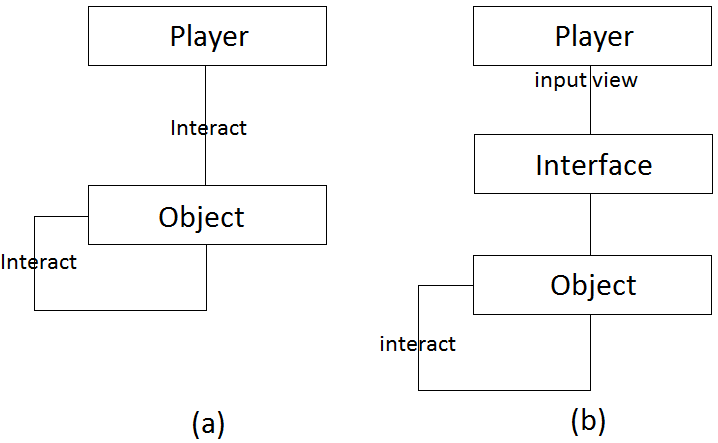
\includegraphics[scale=0.4]{player-object-merged}
\caption[The player-token interaction]{(a) Gameplay independent of player experience, (b) Gameplay depended of player experience (modiefied from \cite{umlapproach})}
\label{fig:playerobject}
\end{center}
\end{figure} 


As a part of gameplay there is a user interface. The interface is necessary to enable interaction between the player and the object. In \cite{umlapproach} Siang et al. present a figure describing the gameplay, see Figure \ref{fig:playerobject} (b). The interface is where and with what the player interacts with the game and includes the input that is sent through the input devices, like a game control, and the output the user receives on the screen and through the speakers \cite{umlapproach}.

\subsection{Story}
One important element of a video game is the story, or the narrative. The story is included in the game to make the involvement and enjoyment better for the player. The story is just a part of the game, and is not the game \cite{umlapproach}.  Different events make up the narrative and will usually contain settings and characters \cite{understandingvg}. Unlike literature and film, which centers on the story, the game centers on play. Therefore, the narrative should be looked at in a player-centric context \cite{gametheory}. Players often make their own story throughout the game \cite{umlapproach}. This means that the game designer creates the background storyline, while the player creates the experimental story while interacting with the game or others. 

In \cite{understandingvg} they introduce interesting elements of the narrative in a video game, and discuss three different categories: \emph{The fictional world}, \emph{Mechanics}, and \emph{Reception}.

\subsubsection{The fictional world}
\label{subsub:fictionalworld}
This category includes settings and actors, which can also be thought of as the \emph{what} and \emph{who}. In \cite{beram}, this is described as objects. Objects are defined as the elements that form the gameplay by adding depth, atmosphere and interactivity to the setting. The \emph{setting}, or \emph{location} as called in \cite{beram}, can also be considered as an object. The setting will be described later in this section.

\cite{beram} defines three categories of objects:
\begin{itemize}
\item \emph{Structural-objects (static):} These objects do not change visually and are in the game to add functionality. Examples are trees, table, walls.
\item \emph{Interactive-objects/entities (dynamic):} These objects will react to the input from the player and other events in the game and will add more functionality to the game. The character is an example of an interactive-object.
\item \emph{Scripting-objects (behaviour):} These objects are not physical, but they are conceptual parameters that adds functionality to the the other object-types. The parameters say something about how the objects will react to events. One example is a game manager that contains parameters like number of life and high scores \cite{umlapproach}. 
\end{itemize}

The game space, which is the \emph{game setting} or \emph{location}, is an important part of a game. The game space is a reproduction of some of the features of the real world and contains specific rules to make it possible to play the game. There are different characters in a game. There are both the characters that the game is about and characters that make things happen and that interacts with the main characters. Therefore, all the different characters need to be considered. \cite{understandingvg} proposes four different categories of characters: 

\begin{itemize}
\item \emph{Stage Characters:} These characters can not be interacted with, and serve more as just a part of a scenario. \\
\item \emph{Functional Characters:} These are also just a part of a scenario, but in addition, they have a general function, which makes it possible for the player to interact with them in some way. \\
\item \emph{Cast Characters:} These have specific functions in the game that have something to do with the story. \\
\item \emph{Player Characters:} These are the characters that the player is in control of. 
\end{itemize}

The different characters can be constructed in different ways. They can be constructed through description, which means through the way we can see them on the screen. This can be done in a symbolic, naturalistic or a "real-life" way. See Table \ref{tab:description} for examples.

\begin{table}
\centering
    \begin{tabular}{|l|l|}
        \hline
        \textbf{Type of description} & \textbf{Example} \\ \hline
       Symbolic & Red haired girl is diabolic  \\ \hline
       Naturalistic & Villains are ugly, while heroes are good-looking \\ \hline
       Real-life & David Beckham as a football player \\ \hline
    \end{tabular}
    \caption[Different ways to describe characters]{Different ways to describe characters \cite{understandingvg}.}
    \label{tab:description}
\end{table} 

The characters can also be described through their actions, through their relationship to space, through other character’s views, or just through a meaningful name. The player character is the most important type, and was by Toby Gard divided in three different categories, in accordance to how easy the player will identify with them. The different categories are \emph{avatars}, \emph{actors} and \emph{roleplaying}, and are defined as:

\emph{"Avatars are a non-intrusive representation of ourselves, actors are always part of a story (or have a story, albeit minimal sometimes), and roleplaying characters have very different abilities that we can raise according to our performance"}. \cite{understandingvg}

Usually, the use of avatars implies that the view is in first-person, which means that the avatars can not be seen, while actors usually will be seen in third-person. In addition, actors will usually have a personality and they are well integrated in the story, while an avatar usually do not have a personality at all. Roleplayers are quite different. Here the players create their own characters. The player can choose their name, and their abilities, as well as if they want to play in first-person or third-person.  

\subsubsection{Mechanics}
This category describes how to organise narrative action. There is a basic concept for how to organise the story in a game, which is called "branching". This means to have multiple paths in the story. 

\begin{figure}
\begin{center}
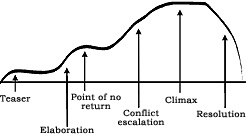
\includegraphics[scale=1.0]{linearFiction}
\caption[Classical linear fiction]{A model of classical linear fiction \cite{understandingvg}}
\label{fig:linearfiction}
\end{center}
\end{figure} 
\begin{figure}
\begin{center}
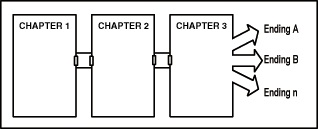
\includegraphics[scale=1.0]{interactiveFiction}
\caption[Interactive fiction]{A model of interactive fiction \cite{understandingvg}}
\label{fig:interactivefiction}
\end{center}
\end{figure} 

Figure \ref{fig:linearfiction} shows the standard progression of a story of linear fiction. In traditional stories, it goes through a resolution. This can not be applied in a game, because it would not let the player do anything. Therefore, a model of interactive fiction is applied for a game. As shown in Figure \ref{fig:interactivefiction}, this model has no continuous curve. In this model it is more about finishing each chapter by solving puzzles, and it relies on the emotional satisfaction the player gets from the victory of solving a puzzle. Even though an action in a game can lead to different endings, the player is actually solving a story. These games are called \emph{progression games} because the player has to finish different actions and chapters, before proceeding. The different chapters are cumulative, meaning that each chapter are building on each other. It is very common in these kind of games that it is a climax or a resolution at the end of each chapter (for example "fight the boss", which is quite common in many games). 

The other structure of narratives, is \emph{emergence games}. This structure depends on a more active artificial intelligence where all the objects in the game have behaviours. To understand the difference between progression games and emergence games we provide an example directly drawn from \cite{understandingvg}: \emph{"In a progression game, the dragon will always attack the player when she steps into the cave, but in an emergence game, this might depend on how the player behaves towards the dragon, which is a more "active" object with a few possible different responses."} 

To be able to easily explore the smaller events in a game, game designers are making so called "quests", which is the missions players have to perform in the game. When the different quests are defined, it can be put together and be told as a story. In \cite{understandingvg} they say that \emph{"ideally, quests are the glue where world, rules and themes come together in a meaningful way".}

In this chapter we have discussed different elements of a video game. These are important elements that need to be studied to understand video games, and can be used both for evaluating existing games, and for developing new games. The elements will be used as a framework for structuring the functional design of the exergame concept. This can be found in Section \ref{sec:functionaldesign}.

